%% Short data paper template
%% Created by Simon Hengchen and Nilo Pedrazzini for the Journal of Open Humanities Data (https://openhumanitiesdata.metajnl.com)

\documentclass{article}
\usepackage[english]{babel}
\usepackage[utf8]{inputenc}
\usepackage{amssymb}
\usepackage{amsmath}
\usepackage{amsthm}
\usepackage{johd}
\usepackage{braket}
\usepackage{multicol}
\usepackage{todonotes}
\usepackage{graphicx}

\newtheorem{theorem}{Theorem}
\newtheorem{lemma}[theorem]{Lemma}
\newtheorem{definition}[theorem]{Definition}
\newtheorem{proposition}[theorem]{Proposition}
\newtheorem{corollary}[theorem]{Corollary}
\newtheorem{thesis}[theorem]{Thesis}
\newtheorem{example}[theorem]{Example}

\newcommand{\N}{\mathbb{N}}
\newcommand{\R}{\mathbb{R}}
\newcommand{\C}{\mathbb{C}}
\newcommand{\D}{\mathbb{D}}
\newcommand{\DC}{\mathbb{DC}}
\newcommand{\GD}{\mathbb{GD}}
\newcommand{\GDC}{\mathbb{GDC}}
\newcommand{\Z}{\mathcal{O}_\e}
\newcommand{\e}{\epsilon}

\newcommand{\E}{\mathcal{E}}
\newcommand{\F}{\mathcal{F}}
\newcommand{\G}{\mathcal{G}}
\newcommand{\til}{\widetilde}
\renewcommand{\bar}{\overline}

\renewcommand{\Re}{\operatorname{Re}}
\renewcommand{\Im}{\operatorname{Im}}
\newcommand{\Sig}{\operatorname{Sig}}
\newcommand{\Inf}{\operatorname{Inf}}

\newcommand\dstate[2]{\frac{\mathrm{d}\ket{#1}}{\mathrm{d}#2}}

\newcommand\ketbra[2]{\ket{#1}\!\bra{#2}}

\newcommand{\norm}[1]{\left\lVert#1\right\rVert}

\title{Quantum mechanics over dual-complex numbers}

\author{Nathan Houyet$^{a}$, Dogukan Bakircioglu$^{b}$, Pablo Arrighi$^{b}$ \\
        \small $^{a}$Université Paris-Saclay (student), France \\
        \small $^{b}$QuaCS, LMF, France \\
}
\date{}

\begin{document}
\maketitle

\section{Introduction}

We replace the complex field by the dual-complex ring in the postulates of quantum mechanics. This modification allow us to linearly approximate the action of families of quantum operations $\E_z(\rho)$ parametrized by a complex number $z$.

These numbers are of the form $z + t \e$ where $\e^2 = 0$ and $z$ and $t$ are complex numbers. Intuitively $t\e$ symbolizes a small variation of $z$. Dual-complex numbers have found wide applications in automatic differentiation, mechanics and geometry. \cite{brodsky2000, baydin2018, yang1963, rev2016} Recent works have begun to extend our knowledge of dual-complex linear operators. \cite{qi2024, liu2025}

In this paper, we build upon these developments by formulating a self-consistent set of postulates that extend conventional quantum theory into the realm of dual-complex numbers. We introduce translation rules that allow for efficient mapping between the dual-complex and conventional formalisms of quantum mechanics. Some of our results extend what was previously known about dual-complex unitary operators. These technical results may be of independant mathematical interest.

We argue that our extension is physical and offers a rigourous framework for a widely used but often informal technique in physics—the neglect of higher-order terms in functional expansions. Since $\e^2=0$, the algebra of dual-complex numbers encodes first-order approximations, making it well-suited for modelling systems where higher-order effects should be neglected. We provide an example of application of our framework where it allows for an easy derivation of Dirac equation in a family of Quantum Cellular Automata (QCA).

Beyond their technical utility, dual-complex numbers also provide a compelling perspective in foundational debates, particularly the tension between discrete and continuous models of physics. While discrete models are computationally convienient and visually intuitive, continuous models have been more studied and are sometimes easier to work with, especially when symmetries are concerned for instance. This raises the question of whether or not discrete models can fully represent Nature. \cite{kornyak2013, hossenfelder2012, stecker2011, chamseddine2014, chamseddine2017}.
Through our example, we show that the dual-complex framework can has the potential to unify these two perspectives by combining a continuous base field $\C$ with an infinitesimal variation which represents a discrete step. Such an hybrid structure may facilitate smooth translations between continuous and discrete frameworks, potentially offering new tools for quantum computation, simulation and foundations.

Dual-complex numbers constitute a new option in the foundational debate about which set of numbers is needed or useful to express quantum behaviors. Quantum theory based on extension of complex numbers such as quaternion numbers has been known for a long time (\cite{finkelstein1962}) while the debate on the necessity of complex numbers over real numbers is still raging. \cite{hoffreumon2025}

In section 2, we recall all the required notions about dual-complex numbers for later sections. In section 3, we recall a few results about dual-complex linear operators and extend what is known about dual-complex unitary operators. We also define a notion of ordering required for our self-consistency check. In section 4, we use these results to present a set of postulates whose consistency is proved in section 5.
Section 5 we introduce a translation from
Finally, we present an application example in section 6.

\section{Dual numbers}
\noindent Extending real numbers with an imaginary unit $i$ with $i^2 = -1$ gives rise to the complex numbers. Complex numbers form a field and are used in quantum mechanics to represent physical systems and their evolution using complex linear algebra. The set of complex q is $\C = \{a + bi \; | \; a, b \in \R \text{ and } i^2 = 0\}$. If a number $z \in \C$ has the form $z = a + bi$ we denote $a$ the real part and $b$ the imaginary part. We can define the functions $\Re$ and $\Im$ as follows
\begin{multicols}{3}
\noindent
\begin{equation}
\Re: \C \to \R: a + bi \to a
\end{equation}

\columnbreak
\noindent
\begin{equation}
\Im: \C \to \R: a + bi \to b
\end{equation}

\columnbreak
\noindent
\begin{equation}
\forall z \in \C, z = \Re(z) + \Im(z)i
\end{equation}

\end{multicols}

Dual numbers $\D$ were first introduced by \cite{clifford1871} and follow a similar idea. They are generated by introducing an imaginary unit $\e$ with $\e^2 = 0$ to the reals. $\e$ is commuting in multiplication and addition with reals. To avoid confusion with complex, we call the real part of a dual the significant part ($\Sig$) and its imaginary part the infinitesimal part ($\Inf$).

\begin{multicols}{3}
\noindent
\begin{equation}
\Sig: \D \to \R: a + b\e \to a
\end{equation}

\columnbreak
\noindent
\begin{equation}
\Inf: \D \to \R: a + b\e \to b
\end{equation}

\columnbreak
\noindent
\begin{equation}
\forall d \in \D, d = \Sig(d) + \Inf(d)\e
\end{equation}

\end{multicols}

Extending the real numbers with both $i$ and $\e$ gives rise to dual-complex numbers $\DC$. We can see the complex, dual and dual-complex numbers as quotient rings:

\begin{multicols}{3}

\noindent
\begin{equation}
\C \approx \R [i]/\langle i^2+1 \rangle
\end{equation}

\columnbreak

\noindent
\begin{equation}
\D \approx \R [\e]/\langle \e^2 \rangle
\end{equation}

\columnbreak

\noindent
\begin{equation}
\DC \approx \C [\e]/\langle \e^2 \rangle
\end{equation}
\end{multicols}

Alternatively, dual-complex (resp. dual) numbers can be seen as the subalgebra of the matrices of the form

\begin{equation}
\begin{pmatrix}
 a & b\\
 0 & a
\end{pmatrix}
\end{equation}

Where $a, b \in \C$ (resp. $a, b \in \R$). Dual and dual-complex numbers are used in automatic differentiation as they allow to ``cut'' the Taylor expansion from the second term. \cite{baydin2018, rev2016}

\begin{equation}
f(z + \e) = f(z_0) + \e f'(z_0) + \e^2 f''(z_0)/2 + \dots = f(z_0) + \e f'(z_0).
\end{equation}

Higher-order versions of dual-numbers were developed to deal with higher-order derivative. See \cite{szi2021, behr2019}.

\subsubsection*{Ring operations and inversion on dual-complex numbers}

Addition and multiplication are defined as follows:

\begin{equation}
(z_1 + t_1 \e) + (z_2 + t_2 \e) = (z_1 + z_2) + (t_1 + t_2) \e
\end{equation}

\noindent \begin{equation}
(z_1 + t_1 \e) (z_2 + t_2 \e) = (z_1 z_2) + (t_1 z_2 + z_1 t_2) \e
\end{equation}

Notice how with the infinitesimal unit $z_2 t_2 \e^2$ vanish into oblivion when with the imaginary unit it becomes real and negative.

A dual-complex is called infinitesimal when its significant part is zero. The set of infinitesimal dual-complex numbers is denoted $\Z = \{0 + t \e | t \in \C\} = \e \C$. A number that is not infinitesimal is called appreciable. We can observe three cases when dividing $w_1 = z_1 + t_1 \e$ by $w_2 = z_2 + t_2 \e$:

\begin{enumerate}
        \item When $w_2$ is appreciable, i.e.\ $z_2 \neq 0$. In this case, the inverse of $w_2$ exists and division is defined as
        \begin{equation}
        \frac{z_1 + t_1 \e}{z_2 + t_2 \e} = \frac{(z_1 + t_1 \e)(z_2 - t_2 \e)}{(z_2 + t_2 \e)(z_2 - t_2 \e)} = \frac{z_1 z_2 - z_1 t_2 \e + t_1 z_2 \e}{z_2^2} = \frac{z_1}{z_2} + \frac{z_2 t_1 - z_1 t_2 }{z_2^2} \e
        \end{equation}
        \item $z_2 = 0$ and we divide the infinitesimal part ($z_1 = 0$). The usual constraint that $w' = \frac{w_1}{w_2} \iff w'w_2 = w1$ leaves us (infinitely) many solutions. Let's say that we want to find $w' = z' + t'$, the quotient of $w_1$ and $w_2$.
        \begin{equation}
        z' + t' \e = \frac{t_1 \e}{t_2 \e} \iff z' t_2 \e + t' t_2 \e^2 = t_1 \e \iff z' = t_1/t_2
        \end{equation}
        There is no constraint on $t'$. However, a natural definition would be $t' = 0$, implying $\frac{t'_1 \e}{t'_2 \e} = \frac{t'_1}{t'_2}$. This is only a convenience definition as $w_2$ has no inverse.
        \item $z_2 = 0$ and we divide the (non-zero) non-dual part $z_1$. In this case we have no solution because $z' + t'\e = \frac{z_1}{t_2 \e} \iff z' t_2 \e = z_1$ which is impossible (by hypothesis $z', t_2, z_1 \in \C$).
\end{enumerate}

Division between $w_1$ and $w_2$ is therefore defined for $w_1$ infinitesimal or $w_2$ appreciable.

Exponentiation and rooting of dual-complex are given by

\begin{proposition}
$(z + t\e)^n = z^n + n z^{n-1} t \e$
\end{proposition}
\begin{proof}
$\DC$ is a commutative ring and therefore the binomial theorem holds.

\noindent \begin{equation}
(z + t\e)^n = \sum_{k=0}^n \binom{n}{k} z^{n-k}(t\e)^k = z^n + nz^{n-1}t\e + (t\e)^2 \sum_{k=2}^n \binom{n}{k} z^{n-k}(t\e)^{k-2} = z^n + nz^{n-1}t\e
\end{equation}
\end{proof}

\begin{corollary}
$\sqrt[n]{z + t \e} = \sqrt[n]{z} + (\frac{t}{n(\sqrt[n]{z})^{n-1}}) \e$ for $z \neq 0$.
\end{corollary}

\subsubsection*{Automatic differentiation}

Dual numbers are useful for automatic differentiation. Given an analytic complex-to-complex function $f(z) = \sum_{n=0}^\infty \frac{f^{(n)}(x_0) z^n}{n!}$ on an open set $D$, we extend it by defining $\hat{f}$ on $D + \Z$ as:

\begin{equation}
        \hat{f}(w) \to \sum_{n=0}^\infty \frac{f^{(n)}(0) w^n}{n!}
\end{equation}

\cite{messelmi2015} proves we can always extend a complex analytic to complex-dual numbers like this.
The usefulness of dual numbers for differentiation comes from the following result:

\begin{proposition}[Automatic differentiation]\label{pr:auto}
        Given $f(z)$, a function from complex to complex which is polymorphic on an open set $D$, there exists a unique polymorphic function $\hat{f}(w)$ defined on $D + \Z$ that agrees with $f(z)$ for every $w \in D$. This function $\hat{f}$ is given by
\begin{equation}
        \hat{f}(z + t\e) = f(z) + t \e f'(z)
\end{equation}
for $z \in D$ and $t \in \R$.
\end{proposition}
\begin{proof}
The following proof being simplified and only meant for intuition, see \cite{messelmi2015} for a full formal proof.\ Given $f(z) = \sum_{n=0}^\infty \frac{f^{(n)}(z_0)(z-z_0)^n}{n!} $ and $\hat{f}(z+t\e)$ agreeing with $f$ for complex values and polymorphic on $D+\Z$, we have, by proposition 1,
\begin{equation}
\begin{split}
        \hat{f}(z + t \e) &= \sum_{n=0}^\infty \frac{\hat{f}^{(n)}(z_0) ((z-z_0) + t\e)^n}{n!}
                           = \sum_{n=0}^\infty \frac{f^{(n)}(z_0) ((z-z_0)^n + n(z-z_0)^{n-1}t\e)}{n!} \\
\end{split}
\end{equation}

Which can be rewritten as

\begin{equation}
\begin{split}
        \hat{f}(z + t \e) &= \sum_{n=0}^\infty \frac{f^{(n)}(z_0) (z-z_0)^n}{n!} + \sum_{n=0}^\infty \frac{f^{(n)}(z_0) n(z-z_0)^{n-1}t\e}{n!} \\
                          &= f(z) + t \e (\sum_{n=0}^\infty \frac{f^{(n)}(z_0) (z-z_0)^n}{n!})' \\
                          &= f(z) + t \e f'(z). \\
\end{split}
\end{equation}
\end{proof}

\begin{corollary}\label{corr:elsc} Dual-complex exponential, logarithm, sine and cosine are given by

\begin{multicols}{2}
\noindent \begin{equation}\label{eq:expscalar}
 \exp(z + t\e) = \exp(z)(1 + t\e)
\end{equation}

\noindent \begin{equation}
 \log(z + t\e) = \log(z) + \frac t z \e
\end{equation}

\columnbreak
\noindent \begin{equation}
 \sin(z + t\e) = \sin(z) + \cos(z)t\e
\end{equation}

\noindent \begin{equation}
 \cos(z + t\e) = \cos(z) - \sin(z)t\e
\end{equation}
\end{multicols}
\end{corollary}

\section{Linear algebra over dual-complex numbers}

In this section, we recall known and introduce new properties of $\D$ and $\DC$ required to show the consistency of our extension of quantum mechanics' postulates to dual-complex numbers in section 4.

We first introduce in section 3.1 an ordering on dual numbers that will be needed to define a set of valid probabilities. In section 3.2, we motivate a choice of conjugation and norm on $\DC$, establish some properties about them before recalling results about diagonalization of dual-complex Hermitian operators. Finally, we establish that dual-complex unitary operators are also diagonalizable and establish their relation to dual-complex skew-Hermitian operators in the sense that they are the exponential and logarithm of each other.

\subsubsection*{Ordering dual and dual-complex numbers}

We know that while $\R$ can be ordered consistently with the field operations, this is not the case for $\C$. Indeed if $\C$ could be totally ordered we would have either $i \geq 0$ or $-i \geq 0$ and then $(\pm i)^2 = -1 \geq 0$. Orderability of $\D$ depends on the definition of an ordered ring, we choose the usual one: a binary relation $\leq$ such that for all $a, b$ in the ring $a \leq b \implies a + c \leq b + c$ and $0 \leq a, 0 \leq b \implies 0 \leq ab$. \cite{fuchs1963} It turns out that there is a very natural lexicographic ordering for $\D$.

\begin{proposition}
 $\D$ can be totally ordered w.r.\@ to $\R$'s natural ordering and this order is unique up to $\pm \e > 0$.
\end{proposition}
\begin{proof}
Suppose $\leq_\D$ is a total ring order on $\D$ such that for any $a, b \in \R$, $a \leq b \iff a \leq_\D b$. Since $\R[\e] \approx \R[-\e]$ we say wlog that $\e \geq 0$. Now aiming at contradiction, suppose that for some $a \in \R^+$ we have $a \leq \e$. Then, $a^2 \leq \e^2 = 0$ which is a contradiction, implying that for every $a \in \R^+$, $a \geq \e$. This is equivalent to say that $\leq_\D$ is a lexicographic order, i.e.\

\begin{equation}
a_1 + b_1 \e \leq_\D a_2 + b_2 \e \iff a_1 < a_2 \lor (a_1 = a_2 \land b_1 \leq b_2)
\end{equation}

This ordering is total and it is easily seen that it is a ring ordering.
\end{proof}

\subsubsection*{Linear algebra}

\noindent Conjugation for hypercomplex numbers of dimension 2 and imaginary unit $X$ is given by $\bar{a + bX} = a - bX$. For dual-complex, we use the complex conjugation as in \cite{qi2023}. We quickly justify this choice by looking at alternative definitions.

\cite{messelmi2015} suggests four different possible conjugations of interest for us

\begin{multicols}{4}
\noindent \begin{equation}
\bar{w} = \bar{z} + \bar{t}\e
\end{equation}

\columnbreak

\noindent \begin{equation}
\til{w} = z - t\e
\end{equation}

\columnbreak

\noindent \begin{equation}
\bar{\til{w}} = \bar{z} - \bar{t}\e
\end{equation}

\columnbreak

\noindent \begin{equation}
w^* = \bar{z}(1-t\e/z)
\end{equation}
\end{multicols}

$w^*$ is the only possible conjugation that satisfies both $w^*w \in \R$ and $\Re(\Sig(w)) = \Re(\Sig(w^*))$. It is, however, non-linear. Our purpose being to extend quantum mechanics with a unit for infinitesimal variations, this conjugation is unfortunate. The choice of $\bar{w}$ over $\til{w}$ and $\bar{\til{w}}$ is motivated by the idea that we can accept a dual norm as $\e$ represents an infinitesimal variation of it, but not a complex norm.

\begin{definition}
For $n \in \N$, $\DC^n$ represents the module of vectors of length $n$ over $\DC$ equipped with an inner-product:
\begin{equation}
 \braket{\psi|\phi} = \sum_k \bar{\psi_k}\phi_k
\end{equation}

\end{definition}

The norm $|w|$ of $w = z + t\e$ is defined as $|w| = \sqrt{w^* w}$. We can observe the following properties

\begin{multicols}{3}
\noindent \begin{equation}
\bar{w_1 + w_2} = \bar{w_1} + \bar{w_2}
\end{equation}

\noindent \begin{equation}
w + \bar{w} = 2 \Re(z) + 2 \Re(t) \e
\end{equation}

\noindent \begin{equation}\label{eq:eq0}
|w| = 0 \iff z = 0
\end{equation}

\columnbreak

\noindent \begin{equation}
\bar{w_1  w_2} = \bar{w_1} ~ \bar{w_2}
\end{equation}

\noindent \begin{equation}\label{eq:sqnorm}
\bar{w}w = |z|^2 + 2 \Re(z\bar{t}) \in \D
\end{equation}

\noindent \begin{equation}\label{eq:geq0}
|w| \geq 0
\end{equation}

\columnbreak

\noindent \begin{equation}
\bar{\bar{w}} = w
\end{equation}

\noindent \begin{equation}\label{eq:modul}
|w| = \sqrt{\bar{w}w} = |z| + \frac{Re(z\bar{t})}{|z|}
\end{equation}

\end{multicols}

In particular equations \ref{eq:geq0} and \ref{eq:modul} entails the following propositions.

\begin{proposition}
 For every $\ket{\psi_\e} = \ket{\psi} + \e \ket{\phi} \in \DC^n$, $\braket{\psi_\e|\psi_\e} = \braket{\psi|\psi} + 2\Re(\braket{\psi|\phi}) \e$ and therefore
\begin{equation}\label{eq:norm}
 ||\ket{\psi_\e}|| = \sqrt{\braket{\psi_\e|\psi_\e}} = ||\ket\psi|| + \frac{\Re(\braket{\psi|\phi})}{||\ket\psi||}\e.
\end{equation}
\end{proposition}
\begin{proposition}
 For any $\ket{\psi} \in \DC^n$, $||\ket\psi|| = \sum_{k=1}^n \psi_k^* \psi_k \geq 0$.
\end{proposition}

A vector in $\D^n$ or $\DC^n$ is called appreciable when its norm is non-zero or equivalently when at least one of its entries is appreciable. Two vectors are called orthogonal when their inner product is zero and appreciably orthogonal when their inner product is infinitesimal.

We define the adjoint as the transpose conjugate, i.e. $A^\dagger = (A^T)^*$. An operator $H$ is Hermitian if it is self-adjoint, i.e.\ $H^\dagger = H$ and skew-Hermitian if $H^\dagger = -H$. An operator is Hermitian (resp.\ skew-Hermitian) if and only if its significant and infinitesimal are Hermitian (resp.\ skew-Hermitian) and $H$ is Hermitian if and only if $iH$ is skew Hermitian.

An operator $U$ is unitary when $U^\dagger U = I$. The following proposition can be derived from this definition.

\begin{proposition}\label{pr:unitary}
The following propositions are equivalent for $U_\e$ a linear operator:

\begin{enumerate}
 \item[a] $U_\e$ is unitary, i.e.\ $U_\e^\dagger U_\e = I$.
 \item[b] $U_\e U_\e^\dagger = I$.
 \item[c] $U_\e$ preserves the inner product, i.e.\ $(U_\e \ket\psi)^\dagger (U_\e \ket\phi) = \braket{\psi|\phi}$ and therefore the norm $||U_\e \ket\psi|| = ||\ket\psi||$.
 \item[d] Rows of $U_\e$ form an orthonormal basis.
 \item[e] Columns of $U_\e$ form an orthonormal basis.
 \item[f] $U_\e = (I + i \e H)U$ where $U$ is a complex unitary and $H$ is a complex Hermitian.
\end{enumerate}
\end{proposition}
\begin{proof}
 For point equivalence between point (f) and (a), let $U_\e = A + B\e$.
\begin{equation}
 \begin{split}
  U_\e^\dagger U_\e = I &\iff A^\dagger A + \e A^\dagger B + \e B^\dagger A = I\\
                        &\iff \begin{cases}
      A^\dagger A = I \\
      A^\dagger B + B^\dagger A = 0
   \end{cases}\\
                        &\iff \begin{cases}
      U := A \text{ is a unitary.} \\
      U^\dagger B = - (U^\dagger B)^\dagger
   \end{cases}\\
 \end{split}
\end{equation}

The second condition can be restated as

\begin{equation}
 \begin{split}
      &U^\dagger B = - (U^\dagger B)^\dagger\\
      \iff &H := i U^\dagger B  \text{ is Hermitian.}\\
      \iff &B = -iUH \text{ and } H \text{ is Hermitian.}
 \end{split}
\end{equation}

Points from (a) to (e) are easily seen to be equivalent by following a reasoning analogous to the one for complex unitary operators which conclude our proof.

\end{proof}

In the rest of this section, we prove that the exponential of dual-complex skew-Hermitian are unitary and the logarithms of a dual-complex unitary are skew-Hermitian. We first introduce the exponential of a dual-complex operator, then recall a known result about dual-complex Hermitian diagonalization and finally introduce two new results about dual-complex unitary operators.

\begin{proposition}
The dual-complex matrix exponential always exists.
\end{proposition}
\begin{proof}
For scalar exponentiation in \ref{eq:expscalar}, we used the dual-complex extension from \ref{pr:auto} which works thanks to binomial theorem and, therefore, commutativity. Commutativity is notoriously not a property of linear operators in general. Without commutativity, we get
\begin{equation}
\exp(A + B \e) = \sum_{n=0}^\infty \frac 1 {n!} (A + B\e)^n = \sum_{n=0}^\infty \frac{A^n}{n!} + \e \sum_{n=0}^\infty \frac 1 {n!} \sum_{k=0}^n \binom n k A^k B A^{n-k}
\end{equation}
The significant part is the exponential of the complex matrix $A$ which is known to always converges. The infinitesimal part also converges as
\begin{equation}
\begin{split}
||\sum_{n=0}^\infty \frac 1 {n!} \sum_{k=0}^n \binom n k A^k B A^{n-k}|| &\leq \sum_{n=0}^\infty \frac 1 {n!} \sum_{k=0}^n \binom n k ||A^k||\, ||B||\, ||A^{n-k}||\\
&\leq ||B||\sum_{n=0}^\infty \frac{2^n ||A||^n}{n!}\\
&= ||B|| \exp(2||A||)
\end{split}
\end{equation}
\end{proof}

A proof identical to that of \cite{liu2025} for the case of dual numbers can be used to show that the exponential of dual-complex matrix $A + B\e$ is $\exp(A) + \e L_{\exp}(A, B)$ where $L_{\exp}(A, B)$ is the Fréchet derivative of the exponential function of $A$ in the direction of $B$.

\begin{proposition}[\cite{qi2021}]\label{pr:qi21}
 Suppose $H$ is a Hermitian operator. Then there exists an orthonormal dual-complex basis $\ket{j_\e}$ and $n$ dual eigenvalues $\lambda_j$ of $H$ such that $H = \sum_j \lambda_j \ketbra{j_\e}{j_\e}$.
\end{proposition}

We now establish that dual-complex unitary operators, just like dual-complex Hermitian operators, are diagonalizable and deduce that their logarithms are Hermitian.

\begin{proposition}[Spectral theorem for dual-complex unitary operators]\label{th:specunit}
 A unitary operator is unitarily diagonalizable, i.e.\ for every dual-complex unitary operator $U_\e$, there is a dual-complex orthonormal basis $\ket{j_\e}$ with associated dual-complex eigenvalues $\lambda_j$ such that $U_\e = \sum_j \lambda_j \ketbra{j_\e}{j_\e}$. These eigenvalues are of the form $e^{i\theta_j} + \e e^{i\theta_j} \mu_j$ where $\theta_j$ and $\mu_j$ are real numbers.
\end{proposition}
\begin{proof}
Let $U_\e = U + i\e U H$ be a dual-complex unitary where $U = \exp(iH_0)$ is a complex unitary operator and $H$ is a Hermitian operator. We are going to build a diagonalizing basis for $U_\e$ from a basis of $H + \e H0$.

By proposition \ref{pr:qi21}, we have that $H_0 + \e H$ is diagonalizable. Let $\ket{j_\e} = \ket{j_1} + \e \ket{j_2}$ be an orthonormal basis in which $H_0 + \e H$ is diagonal. Then, $\ket{j_1}$ also forms an orthonormal basis, and we can uniquely write $H = \sum_{jk} h_{jk} \ketbra{j_\e}{k_\e}$ where $h_{jk}^* = -h{kj}$. Since the eigenvalues of $H_0 + \e H$ are of the form $\theta_j + \e \mu_j$ with $\theta_j, \mu_j \in \R$ we have

\begin{equation}
 H_0 \ket{j_2} + H \ket{j_1} = \theta_j \ket{j_2} + \mu_j \ket{j_1} \iff (H_0 - \theta_j I)\ket{j_2} = (\mu_j I - H) \ket{j_1}
\end{equation}

This implies for each $\ket{k_1}$

\begin{equation}
 \bra{k_1}(H_0 - \theta_j I)\ket{j_2} = \bra{k_1}(\mu_j I - H) \ket{j_1} \iff (\theta_k - \theta_j)\braket{k_1|j_2} = -h_{kj}
\end{equation}

Which implies that for each $j \neq k$ such that $\theta_j = \theta_k$, $h_{jk} = 0$.

We will now be able to prove the following claim: we can always construct an orthonormal basis for $U_\e$, whose significant part is $\ket{j_1}$ and with associated eigenvectors whose significant part is $\lambda_j = e^{i\theta_j}$. We need to find vectors $\ket{j_3}$ and complex values $\sigma_j$ such that

\begin{equation}
 (U - \lambda_j I) \ket{j_3} = (\sigma_j I - iUH) \ket{j_1}
\end{equation}

Where $\lambda_j = e^{i\theta_j}$. Since $U = \sum_{k} \lambda_k \ketbra{k_1}{k_1}$, the left side must necessarily be orthogonal to $\ket{j_1}$ which means

\begin{equation}
 \bra{j_1} (\sigma_j I - iUH) \ket{j_1} = 0
 \iff \sigma_j = i \lambda_j h_{jj} \\
\end{equation}

Let $\ket{j_3} = \sum_j \alpha_{jk} \ket{k_1}$, or, equivalently, let $\alpha_{jk} = \braket{k_1|j_3}$. We find for $k \neq j$

\begin{equation}\label{eq:alphj3}
\begin{split}
 \bra{k_1} (U - \lambda_j I) \ket{j_3} = \bra{k_1} (\sigma_j I - iUH) \ket{j_1}
 \iff& (\lambda_k - \lambda_j) \alpha_{jk} = - i \lambda_j h_{kj}
\end{split}
\end{equation}

When $\lambda_j \neq \lambda_k$. When $\lambda_j = \lambda_k$, we showed that $h_{jk} = 0$ and any value of $\alpha_{jk}$ in $\C$ is a solution. Since we always have $\alpha_{jk}$ satisfying \ref{eq:alphj3}, we have a basis. Consider we choose that $\alpha_{jj} = 0$ and $\alpha_{jk} = 0$ when $\lambda_j = \lambda_k$. It happens that the basis $\ket{j_U} := \ket{j_1} + \e \ket{j_3}$ is orthonormal. Indeed

\begin{gather*}
\alpha_{jk}^* = (\lambda_j \lambda_k) \frac{-i\lambda_j^* h_{jk}}{\lambda_k - \lambda_j} = \frac{-i\lambda_k h_{jk}}{\lambda_k - \lambda_j} = -\alpha_{kj}\\
\implies \braket{j_U|k_U} = \braket{j_1|k_1} + \e \braket{j_3|k_1} + \e \braket{j_1|k_3} = \delta_{jk} + \e (\alpha_{kj}^* + \alpha_{jk}) = \delta_{jk}
\end{gather*}

We now showed that $\ket{j_U}$ is an orthonormal basis and by construction we have $\theta_j, \sigma_j \in \R$ and

\begin{equation}
\begin{split}
\sum_j (\lambda_j + \e \sigma_j) \ketbra{j_U}{j_U} &= (\sum_j e^{i\theta_j} \ketbra{j_1}{j_1}) + \e (\sum_j e^{i\theta_j} \ketbra{j_3}{j_3} + \sigma_j \ketbra{j_1}{j_1})\\
                                                   &= U + i \e UH
\end{split}
\end{equation}
\end{proof}

Thanks to the diagonalization of unitary operators, we can establish the following result.

\begin{proposition}\label{pr:hermunit}
The exponential of Hermitian linear operator is a unitary. Moreover, every unitary $U_\e$ is of the form $\exp(iH)$ where $H$ is Hermitian. $H$ is unique modulo $2\pi$.
\end{proposition}
\begin{proof}
To prove the first statement, let $H$ be a Hermitian operator. Then we have

\begin{equation}
 \exp(iH)^\dagger = (\sum_{n=0}^\infty \frac{(iH)^n}{n!})^\dagger = \sum_{n=0}^\infty \frac{(-iH^\dagger)^n}{n!} = \exp(-iH)
\end{equation}

This shows us that the adjoint of the exponential of $iH$ is its inverse:

\begin{equation}
 \exp(iH)^\dagger \exp(iH) = \exp(-iH) \exp(iH) = \exp(-iH+iH) = \exp(0) = I
\end{equation}

For the second statement, let $U_\e = \sum_j (\lambda_j + \e \sigma_j) \ketbra{j_U}{j_U}$ be a dual-complex unitary operator diagonalized as in proposition \ref{th:specunit}. We can write $\lambda_j + \e \sigma_j = e^{i\theta_j}(1 + i\mu_j)$ where $\theta_j, \mu_j \in \R$. Therefore $\log(U_\e) = \sum_j \log(\lambda_j + \e \sigma_j)\ketbra{j_U}{j_U} = \sum_j (i\theta_j + \e i\mu_j)\ketbra{j_U}{j_U}$ which is indeed skew-Hermitian.

\end{proof}

\begin{corollary}
Let $H_1$ and $H_2$ be complex Hermitian matrices, $L_{\exp}(iH_1, iH_2)$ is of the form $iUH$ where $U$ is unitary and $H$ Hermitian.
\end{corollary}

Another result is required to extend the measurement postulate. We say the operator $E$ is appreciably semipositive if $\braket{\psi|E|\psi}$ positive and appreciable or exactly zero for every vector $\ket\psi$.

\begin{proposition}\label{pr:semipos}
 For every dual-complex linear operator $M_\e$, $M_\e^\dagger M_\e$ is appreciably semipositive.
\end{proposition}
\begin{proof}
Let $\ket\psi$ be an arbitrary vector and $\ket\phi = \sum_j \phi_j \ket{j} = M_\e \ket\psi$ for an orthonormal basis $\ket{j}$. Then $\braket{\psi|M_\e^\dagger M_\e|\psi} = \braket{\phi|\phi} = \sum_j \phi_j^*\phi_j$. From equations \ref{eq:eq0}, \ref{eq:sqnorm} and \ref{eq:geq0} combined, we have that for all $j$, $\phi_j^* \phi_j$ is either appreciable or exactly zero and always greater or equal to zero. It follows that $M_\e^\dagger M_\e$ is appreciably semipositive.
\end{proof}

\section{Postulates of quantum theory over dual-complex numbers}

In this section we introduce an extension of quantum mechnanics postulate to allow for dual-complex amplitudes and operators.
We replace the usual notion of state by that of an ``$\e$-state'', a dual-complex unit vector in the dual-complex extension of a Hilbert-space. We extend the usual notions of unitary evolution and Hermitian observables by allowing dual-complex unitary ``$\e$-evolutions'' and dual-complex Hermitian ``$\e$-observables''.
These notions will allow us to study linear approximation of quantum states, which we will call ``$\e$-quantum states.''.

We present a suggestion of extension of the usual postulates of quantum theory, then justify them quickly.

\paragraph{Postulate 1.} An $\e$-state vector is a unit dual-complex vector. At every time, a dual-complex quantum system is described by an $\e$-state.
\paragraph{Postulate 2.} An operator $U$ represents a valid $\e$-evolution if and only if $U$ is unitary. The evolution of a closed $\e$-quantum system is described by an $\e$-evolution.
\paragraph{Postulate 3.} A set of operators $\{M_m\}$ is an $\e$-measurement operator collection if it is bound by the completeness relation. The evolution of an open $\e$-quantum system is described by such a collection. The outcome $m$ appears with the dual probability $p(m) = \bra\psi M_m^\dagger M_m \ket\psi$. The resulting $\e$-state is

\begin{equation}\label{def:meas}
 \ket{\psi'} = \frac{M_m \ket\psi}{\sqrt{p(m)}}
\end{equation}

\paragraph{Postulate 4.} Given two $\e$-states representing two systems, the composite system is represented by the tensor product of these two $\e$-states.

\subsubsection*{State space}

Postulate 1 aims at capturing the notion of the extension of a state vector to the dual-complex domain. The goal being to take a linear approximation of a system according to a certain parameter, we start at time zero with a usual complex unit vector that we evolve according to postulates 2 and 3, and so our states will always keep a norm equal to $1$.

If we choose to start from a dual-complex vector, since the infinitesimal part of the vector represents the derivative of the significant part according to some parameter, equation \ref{eq:norm} tells us that the norm is one if and only if the derivation operator is skew-Hermitian.

\subsubsection*{Evolution}

This postulate is motivated by the fact that given an analytic path of unitary $U(z)$, its dual-complex extension will be unitary (which is easily seen from the fact that the derivative $U(z)$ is of the form $iU(z)H(z)$ where $H(z)$ is Hermitian). $\e$-evolutions represent therefore a first-order approximation of complex unitary evolutions.

In conventional quantum mechanics, this postulate is equivalently expressed through the Schrödinger equation. From proposition \ref{pr:hermunit}, we can restate our extension of postulate 2 as

\paragraph{Postulate 2'.} The evolution of a closed system is described by the Schrödinger equation,
\begin{equation}
 i\hbar \dstate \psi t = H\ket\psi
\end{equation}

Where $\ket\psi$ is an $\e$-state, $H$ a dual-complex Hermitian linear operator and $\hbar$ is the Planck's constant.

\subsubsection*{Measurement}

Similar to postulate 2, we extend general measurements with dual-complex operators by taking a collection of analytic measurement operators and extend them into $\DC$. It can easily be seen that since $\sum_m M_m^\dagger M_m = I$, their derivatives $\dot{M_m}$ is such that $\sum_m M_m^\dagger \dot{M_m}$ is skew-Hermitian. It can also be seen that for an $\e$-quantum measurement operators collection $\{M_m + \e N_m\}$, the completeness relation $\sum_m (M_m + \e N_m)^\dagger (M_m + \e N_m)$ can be restated as

\begin{multicols}{2}
\noindent \begin{equation}
 \text{(i) } \sum_m M_m^\dagger M_m = I
\end{equation}
\columnbreak
\noindent \begin{equation}
 \text{(ii) } \sum_m M_m^\dagger N_m \text{ is skew-Hermitian.}
\end{equation}
\end{multicols}

The conventional postulate for measurements also defines what are the resulting states and with which probability. To ensure our extension doesn't create unwanted behaviors, we must check that probabilities are positive and sum to one. We must also check that the resulting state is well defined as it is renormalized by a probability that could maybe be infinitesimal. Fortunately, such behaviors do not arise, as we show in the next section (\ref{pr:consistency}).

In particular, as in conventional quantum theory, we can see that when we have exactly one measurement operator, it is a unitary, which means that the extended postulate 2 can be reduced to the postulate 3.

\subsubsection*{Composite systems}

Composing systems is done in the usual, conventional way, using tensor products. Again the postulate preserves the unit norm. If we have two $\e$-states $\ket\psi$ and $\ket\phi$, their norm will be $\sqrt{\braket\psi\psi \braket\phi\phi} = 1$.

\subsubsection*{Density operators formalism}

We use the usual notion of density operators, which is easily seen to be compatible with the extended postulates. An $\e$-density operator $\rho$ is a dual-complex, unit-trace, positive operator. As in the conventional complex case, applying a unitary $U$ to $\rho$ yields $U \rho U^\dagger$ and measuring $\rho$ with $\{M_m\}$ yields $\sum_m M_m \rho M_m^\dagger$.

\section{Consistency of the extended postulates}

In this section, we show that the evolution of a system preserves the norm of the state vector (self-consistency) and that our postulates provide a first-order approximation of quantum systems.

\subsubsection*{Self-consistency}

\begin{proposition}\label{pr:consistency}
A system that starts from an $\e$-states and is evolved by $\e$-evolutions and $\e$-measurements is described by an $\e$-state at all time, i.e.\ if there's a sequence $\ket{\psi_0}, \ket{\psi_1}, \dots, \ket{\psi_k}$ such that $\ket{\psi_0}$ is an $\e$-state and $\ket{\psi_{j+1}}$ was obtained either by applying an $\e$-unitary or an $\e$-measurement to $\ket{\psi_j}$, every $\ket{\psi_j}$ is an $\e$-state. Moreover, probabilities from any $\e$-measurement are either zero or appreciably positive and sum to one.
\end{proposition}
\begin{proof}
By proposition \ref{pr:unitary}, a dual-complex unitary preserves the norm. For measurements, from \ref{def:meas} norm preservation is given by
\begin{equation}
\norm{\frac{M_m \ket\psi}{\sqrt{p(m)}}} = \norm{\frac{M_m \ket\psi}{\sqrt{\braket{\psi|M_m^\dagger M_m|\psi}}}} = \frac{||M_m \ket\psi||}{||M_m\psi||} = 1.
\end{equation}
Probabilities sum to one since $\sum_m p(m) = \sum_m \braket{\psi|M_m^\dagger M_m|\psi} = \braket{\psi|(\sum_m M_m^\dagger M_m)|\psi} = \braket{\psi|I|\psi} = 1$ and are either zero or appreciably positive by proposition \ref{pr:semipos}.
\end{proof}

\subsubsection*{Consistency with conventional quantum theory}

\begin{definition}\label{def:ext}
We introduce the dual-complex extension of a quantum operation and the correction of dual-complex quantum operation.
\begin{itemize}
 \item Let $\E_z(\rho)$ be a quantum operation analytic in $z$ whose operator-sum representation is, for some basis $\ket{e_k}$ and unitary operator $U_z$,
\begin{equation}\label{eq:opsum}
\E_z(\rho) = tr_B(U_z [\rho \otimes \ketbra{e_0}{e_0}] U_z^\dagger)
\end{equation}

Let $\dot{\E_z} = \frac{\mathrm{d}\E_z}{\mathrm{d}z}$. We call $\E$'s dual-complex extension the dual-complex operation

\begin{equation}
\F_{z+\dot{z}\e}(\rho) = \E_z(\rho) + \dot{z}\e \dot{\E}_z(\rho)
\end{equation}

 \item Let $\F_w(\rho)$ be a dual-complex extension of a quantum operation $\E_z(\rho)$ as in \ref{eq:opsum} where $w = z + \dot{z}\e$. Then $\F_w$ has the form
        \begin{equation}
        \F_{w}(\rho) = tr_A(V_w [ \ketbra{e_0}{e_0} \otimes \rho V_w^\dagger)
        \end{equation}
  where $V_w = U_z + \e \dot{z} \dot{U_z}$, $\dot{U_z} = \frac{\mathrm{d}U_z}{\mathrm{d}z} = iU_zH$ and $H$ is Hermitian. $\til{V}_w(h)$ is the complex correction of $V_w$ with parameter $h \in \R$, defined as
        \begin{equation}
        \til{V}_w(h) = U_z + i \dot{z} h {U_z} H + h^2\sum_{n=0}^\infty \frac{1}{n!} (iH)^{n+2}h^n
        \end{equation}
  $\til{\F}_w(\rho, h)$ is the complex correction of $\F_w(\rho, h)$ with parameter $h \in \R$, defined as
        \begin{equation}\label{eq:corrF}
        \til{F}_w(\rho, h) = tr_A(\til{V}_w(h) [ \ketbra{e_0}{e_0} \otimes \rho ] \til{V}_w(h)^\dagger)
        \end{equation}
\end{itemize}

\end{definition}

\begin{proposition}\label{pr:frbk}
Let $\E_z(\rho)$ and $\F_w(\rho)$ be a quantum operation and its dual-complex extension. For any parameter $h \in \R$, the correction $\til{F}_w(\rho, h)$ is a valid quantum operation and $\til{F}_{z + \dot{z}\e}(\rho, h) = \E_z(\rho) + O(h^2)$.
\end{proposition}

\begin{proof}
First, observe that $\til{V}_w(h)$ is a unitary
\begin{equation}
\til{V}_w(h) = U_z + i \dot{z} h U_z H + h^2 \sum_{n=0}^\infty \frac{1}{n!} (iH)^{n+2}h^n = U_z(\sum_{n=0}^\infty \frac{1}{n!} (iHh)^{n}) = U_z \exp(iHh).
\end{equation}

It immediately follows that \ref{eq:corrF} is a quantum operation. For the second claim, we can see that

\begin{equation}
\begin{split}
\end{split}
\begin{align*}
\mathcal{E}_{z+\dot{z}h}(\rho)
&= \mathcal{E}_z(\rho) + \dot{z} h \dot{\mathcal{E}}(\rho) + O(h^2) \\
~
~
\tilde{F}_{z+\dot{z}\e}(\rho, h)
~
&= \operatorname{tr}_A\left(\til{V}_{z+\dot{z}\e}(h) \left[ \ketbra{e_0}{e_0} \otimes \rho \right] \til{V}_{z+\dot{z}\e}(h)^\dagger\right) \\
~
&= \operatorname{tr}_A\left(\left( U_z + \dot{z} h \dot{U}_z + O(h^2) \right)
\left[ \ketbra{e_0}{e_0} \otimes \rho \right]
\left( U_z + \dot{z} h \dot{U}_z + O(h^2) \right)^\dagger\right)\\
~
&=\operatorname{tr}_A\left(U_z \left[ \ketbra{e_0}{e_0} \otimes \rho \right] U_z^\dagger\right) \\
&+ \operatorname{tr}_A\left(U_z \left[ \ketbra{e_0}{e_0} \otimes \rho \right] (\dot{z} h \dot{U}_z)^\dagger
+ (\dot{z} h \dot{U}_z) \left[ \ketbra{e_0}{e_0} \otimes \rho \right] U_z^\dagger \right) + O(h^2)\\
~
&= \mathcal{E}_z(\rho) + \dot{z} h \dot{\mathcal{E}}_z(\rho) + O(h^2)
\end{align*}
\end{equation}
\end{proof}

\begin{example}
We have dual-complex quantum operation $\F(\rho) = \sum_m M_m \rho M_m^\dagger$.

\begin{multicols}{2}
\noindent \begin{equation}
 M_0 = \ketbra 0 0
\end{equation}

\noindent \begin{equation}
 M_1 = \ketbra 0 1
\end{equation}

\columnbreak

\noindent \begin{equation}
 N_0 = i \pi \ketbra 0 0
\end{equation}

\noindent \begin{equation}
 N_1 = i \pi (\frac 1 {\sqrt 3} \ketbra 1 0 + \ketbra 0 1 - \frac 2 {\sqrt 6} \ketbra 1 1)
\end{equation}
\end{multicols}

Our goal is to find a conventional quantum measurement collection $\til M_m(h)$ such that $\til M_m(h) = M_m + h N_m + O(h^2)$. To achieve this, we are going to apply \ref{def:ext} correction. First we need to rewrite $\F(\rho)$ as $tr_A(U_\e \left[ \ketbra{e_0}{e_0} \otimes \rho \right] U_\e^\dagger)$ where $U_\e$ is a dual-complex unitary. By \label{pr:unitary}, we can write $U_\e = U + \e \dot{U}$ where $\dot{U} = iHU$, $U$ is a conventional complex unitary and $H$ is a conventional complex Hermitian.

To determine $U$, we see that the only constraint is that $\ket{m_A} U \bra{0_A} = M_m$ and that the SWAP gate is on that fulfills this condition. We therefore have

\begin{equation}
 U = \begin{pmatrix}
        1 & 0 & 0 & 0 \\
        1 & 0 & 1 & 0 \\
        0 & 1 & 0 & 0 \\
        0 & 0 & 0 & 1 \\
     \end{pmatrix}
\end{equation}

To find a correct value for $\dot{U}$, we can use that its first two columns are defined by $N_m$ and that $U^\dagger\dot{U}$ must be Hermitian. Using this we can find the first two columns of $U^\dagger\dot{U}$ and complete the rest of the matrix to make it Hermitian. We eventually can find, among other possible solutions, $H$ defined by

\begin{equation}
 H = \frac \pi {\sqrt 6} \begin{pmatrix}
        \sqrt{6} & 0 & 0        & -\sqrt 2 \\
        0        & 0 & 0        & 0        \\
        0        & 0 & \sqrt{6} & -2       \\
        -\sqrt 2 & 0 & -2       & \sqrt{6} \\
     \end{pmatrix}
\end{equation}

Then our corrections are defined by $\til M_m(h) = \ket{m_A} \exp(iH) U \bra{0_A}$ which is given by

\begin{equation}
 \til M_0(h) = \frac 1 6 \begin{pmatrix}
         4e^{i \pi h} + e^{i \pi 2 h} + 1 & \sqrt 2 (2 e^{i \pi h} - e^{i \pi 2 h} - 1) \\
         0 & 0
     \end{pmatrix}
\end{equation}

\begin{equation}
 \til M_0(h) = \frac 1 6 \begin{pmatrix}
         \sqrt 2 (2 e^{i \pi h} - e^{i \pi 2 h} - 1) & 2(e^{i \pi h} + e^{i \pi 2 h} + 1) \\
         \sqrt{3}(e^{i \pi 2 h - 1}) & \sqrt{6} (1 - e^{i \pi 2 h})
     \end{pmatrix}
\end{equation}

And have $\til \F_h(\rho) = \sum_m \til M_m(h) \rho \til M_m(h)^\dagger$, a valid convention quantum operation.

\end{example}

\section{Application example: Quantum Cellular Automata}

In this section, we apply the dual-complex extension of quantum operations to a quantum walk. We first explain the quantum walk from \cite{arrighi2020} which simulates the movement of a fermion using discrete time and space. This discrete model exactly obeys the Dirac equation with an error term. We extend the quantum operation defined by this walk to the dual-complex and derive exactly the Dirac equation, hereby creating a bridge between a discrete and a continuous model of the fermion.

The quantum walk represents a fermion moving either left or right. Space and time are made discrete with a step $h$. At each step, the fermion can either continue in the same direction or change its direction with an amplitude depending of its mass. $\ket{x+}$ and $\ket{x-}$ represents respectively a fermion moving right and left and the state of our fermion at time $t$ is given by $\ket{\psi(t)} = \sum_x \psi^+(x, t)\ket{x+}+\psi^-(x, t)\ket{x-}$. The relation between the amplitudes at step $t$ and at step $t+h$ is given by

\begin{equation}
 \begin{pmatrix}
  \psi^+(x, t + h) \\
  \psi^-(x-h, t + h)
 \end{pmatrix} = W \begin{pmatrix}
  \psi^-(x, t) \\
  \psi^+(x-h, t)
 \end{pmatrix}
\end{equation}

where $W$ is a gate defined by

\begin{equation}
W = W_h = \begin{pmatrix}
-i\sin(mh) & \cos(mh) \\
\cos(mh) & -i\sin(mh) \\
\end{pmatrix}
\end{equation}

Figure \ref{fig:diracqca} shows how $W$ acts on two sites and how the wires are then crossed. The action of these gates followed by the wire crossing defines a unitary action $U$ relating the state of the system at step $t$ and at step $t + h$.

\begin{figure}[htp]
\centering

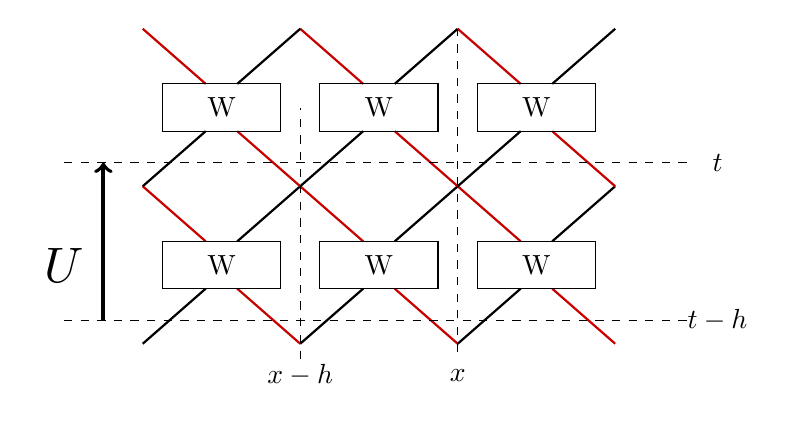
\begin{tikzpicture}[scale=1, every node/.style={scale=1}]
% Define colors
\definecolor{red}{RGB}{200,0,0}

\foreach \x in {-1, 0, 1}
        \foreach \y in {0, 1} {
                \draw[black, thick] (2+2*\x,-1+2*\y) -- ++(1-.2, 1-.3);
                \draw[red, thick] (2+2*\x, 1+2*\y) -- ++(1-.2, -1+.3);
}
\foreach \x in {0, 1, 2}
        \foreach \y in {0, 1} {
                \draw[red, thick] (2+2*\x,-1+2*\y) -- ++(-1+.2, 1-.3);
                \draw[black, thick] (2+2*\x, 1+2*\y) -- ++(-1+.2, -1+.3);
}

\draw[black, dashed] (2, -1.2) -- (2, 2);
\draw[black, dashed] (4, -1.1) -- (4, 3);
\draw[black, dashed] (-1, -0.7) -- (7, -0.7);
\draw[black, dashed] (-1, 1.3) -- (7, 1.3);

\node at (2, -1.4) {$x-h$};
\node at (4, -1.4) {$x$};

\node at (7.3, 1.3) {$t$};
\node at (7.3, -0.7) {$t-h$};

% Rectangles (quantum gates)
\node[draw, minimum width=1.5cm, minimum height=0.6cm] at (1,0) {W};
\node[draw, minimum width=1.5cm, minimum height=0.6cm] at (3,0) {W};
\node[draw, minimum width=1.5cm, minimum height=0.6cm] at (5,0) {W};
\node[draw, minimum width=1.5cm, minimum height=0.6cm] at (1,2) {W};
\node[draw, minimum width=1.5cm, minimum height=0.6cm] at (3,2) {W};
\node[draw, minimum width=1.5cm, minimum height=0.6cm] at (5,2) {W};

\node[scale=1.8] at (-1, 0) {$U$};
\draw[->, line width=1.4pt] (-.5, -.7) -- ++(0, 2);
\end{tikzpicture}

    \caption{Dirac QCA}
    \label{fig:diracqca}
\end{figure}

The global action of the walk at each step is a unitary $U =  U_h$ consisting of the tensor product of all the $W$ gates composed with the wires crossings. Since the wires crossings do not depend on $h$, we can compute the dual-complex extension of $U$, call it $U_\e$, by simply extending $W$. From \ref{corr:elsc}, we get

\begin{equation}
W_\e = \begin{pmatrix}
-im\e & 1 \\
1 & -im\e \\
\end{pmatrix}
\end{equation}

By \ref{pr:auto}, we can see we have

\begin{equation}
\begin{split}
  &\psi^+(x, t+\e) = \psi^+(x-\e, t) - im\e \psi^-(x, t) \\
  \implies &\psi^+(x, t) + \e \frac{\partial}{\partial t}\psi^+(x, t) = \psi^+(x, t) - \e \frac{\partial}{\partial x} \psi^+(x, t) - im\e \psi^-(x, t) \\
  \implies & \frac{\partial}{\partial t}\psi^+(x, t) = - \frac{\partial}{\partial x} \psi^+(x, t) - im \psi^-(x, t) \\
 \end{split}
\end{equation}

\begin{equation}
\begin{split}
   &\psi^-(x, t+\e) = \psi^-(x+\e, t) - im\e \psi^+(x, t) \\
  \implies &\psi^-(x, t) + \e \frac{\partial}{\partial t}\psi^-(x, t) = \psi^-(x, t) + \e \frac{\partial}{\partial x} \psi^-(x, t) - im\e \psi^+(x, t) \\
  \implies & \frac{\partial}{\partial t}\psi^-(x, t) = \frac{\partial}{\partial x} \psi^-(x, t) - im \psi^+(x, t) \\
 \end{split}
\end{equation}

These two equations can be rewritten in a condensed form which is equivaelent to the Dirac equation.

\begin{equation}
 \partial_t \psi = - \sigma_3 \partial_x \psi - im \sigma_1 \psi
\end{equation}

\begin{equation}
\begin{split}
 &(i(\sigma_1, \sigma_1 \sigma_3)^T \cdot (\partial_t, \partial_x) - mI) \psi(x, t) = 0 \\
 &\implies (i \gamma^J \partial_J - m) \psi = 0
\end{split}
\end{equation}

where
\begin{equation}
 \psi(x, t) = \begin{pmatrix}
         \psi^+(x, t)\\
         \psi^-(x, t)\\
        \end{pmatrix}
\end{equation}

By \ref{pr:frbk}, it follows that as $h$ goes to zero, so does $h^2$ and therefore this quantum walk converges to a Dirac equation.

Finally, we can complete this example by applying \ref{def:ext} and construct the correction of $W_\e$, $\til{W}_\e(h)$. Indeed, $W_\e$ is not a unitary in the conventional sense, so we can apply our correction get one. By following the process of \ref{eq:corrF}, we get.

\begin{equation}
\til{W}_\e(h) = W_h = \begin{pmatrix}
-i\sin(hm) & \cos(hm) \\
\cos(hm) & -i\sin(hm) \\
\end{pmatrix}
\end{equation}


\section{Conclusion}

In this paper, we demonstrated how extending quantum mechanics from complex numbers to dual-complex numbers can offer a fruitful bridge between continuous and discrete models.

First, we advanced our knowledge of dual-complex linear algebra by demonstrating that dual-complex unitary are 1) diagonalizable and 2) related to dual-complex Hermitian \textit{via} exponentiation and logarithm maps. We also introduced a notion of ordering on dual-complex numbers along with one of dual-complex semipositive operators.

Second, we presented a set of postulates extending quantum mechanics by introducing an infinitesimal unit $\e$ satisfying $\e^2 = 0$. We establihed its self-consistency by showing norm and probabilities preservation, and showed that the equivalence between the Schrödinger's equation and unitary formulation of evolution of quantum system continues to hold in dual-complex quantum systems.

Third, we introduced a translation between conventional and dual-complex quantum operation families, and proved these translations preserve the action of the operation up to the terms of order $O(h^2)$.

Fourth, we applied these translations to a concrete example, ultimately deriving the Dirac equation in the dual-complex formalism from a discrete quantum walk.

These results show the possibility and usefulness of applying dual-complex numbers to quantum theory. They are also of general mathematical interest as they contribute to the ongoing research on dual-complex linear operators.

Future explorations could extend these translations to construct explicit bridges between discrete and continuous models in quantum mechanics. Additionnaly, the foundational debate on the set of numbers to use for quantum mechanics could also benefit of generalization of our extension to higher-order dual-complex numbers or general quaternions $H(\alpha, 0)$. An other direction would be to explore connections with Grassman numbers, which also obeys nilpotency conditions and may offer new ways of describing fermionic systems in a generalized dual-complex formalism of quantum mechanics.

\bibliographystyle{johd}
\bibliography{bib}

\end{document}
